\chapter{Hyper-parameter tuning} \label{app:hyperparameter_tuning}

\section{Hyper-parameter search space} \label{app:hyperparameter_search_space}

For the five implemented \acrlong{drl} algorithms, Table \ref{tab:model_hyperparameters} summarises the hyper-parameters that were tuned during the training process.

\chapter{Hyper-parameter tuning} \label{app:hyperparameter_tuning}

For the five implemented \acrlong{drl} algorithms, the following table summarises the hyper-parameters that were tuned during the training process.

\begin{table}[h!]
\centering
\begin{tabular}{|l|l|p{8cm}|}
\hline
\textbf{Model} & \textbf{Hyperparameter} & \textbf{Values / Range} \\ \hline
\multirow{3}{*}{\textbf{A2C}} 
 & Number of steps & \{5, 10, 20, 30, 40\} \\
 & Entropy coefficient & Uniform[1$\times$10$^{-8}$, 1$\times$10$^{-3}$] \\ 
 & Learning rate & Uniform[1$\times$10$^{-5}$, 1$\times$10$^{-2}$] \\ \hline

\multirow{4}{*}{\textbf{PPO}} 
 & Number of steps & \{128, 256, 512, 1024, 2048\} \\ 
 & Entropy coefficient & Uniform[1$\times$10$^{-8}$, 1$\times$10$^{-3}$] \\ 
 & Learning rate & Uniform[1$\times$10$^{-5}$, 1$\times$10$^{-2}$] \\ 
 & Batch size & \{32, 64, 128, 256, 512\} \\ \hline

\multirow{3}{*}{\textbf{DDPG}} 
 & Batch size & \{64, 128, 256\} \\ 
 & Buffer size & \{50000, 100000, 200000, 500000\} \\ 
 & Learning rate & Uniform[1$\times$10$^{-5}$, 1$\times$10$^{-2}$] \\ \hline

\multirow{3}{*}{\textbf{TD3}} 
 & Batch size & \{64, 100, 128, 256\} \\ 
 & Buffer size & \{500000, 1000000, 2000000\} \\ 
 & Learning rate & Uniform[1$\times$10$^{-5}$, 1$\times$10$^{-2}$] \\ \hline

\multirow{5}{*}{\textbf{SAC}} 
 & Batch size & \{32, 64, 128\} \\ 
 & Buffer size & \{100000, 500000, 1000000, 2000000\} \\ 
 & Learning rate & Uniform[1$\times$10$^{-5}$, 1$\times$10$^{-2}$] \\ 
 & Learning starts & \{500, 1000, 2000, 5000\} \\ 
 & Entropy coefficient & \{"auto", "auto\_0.1", "auto\_0.01"\} \\ \hline
\end{tabular}
\caption{Hyperparameter configurations for different RL algorithms.}
\label{tab:model_hyperparameters}
\end{table}

\section{Default Hyper-parameter Configuration} \label{app:default_hyperparameters}

In addition, the default hyper-parameter configuration is shown in Table \ref{tab:default_hyperparameters}.
\begin{longtable}{|l|l|p{8cm}|}
    \caption{Default hyper-parameter configurations.}
    \label{tab:default_hyperparameters}
    \\ 
    \hline
    \textbf{Model} & \textbf{Hyperparameter} & \textbf{Values / Range} \\ \midrule
    \endfirsthead

    \hline
    \textbf{Model} & \textbf{Hyperparameter} & \textbf{Values / Range} \\ \midrule
    \endhead

    \endfoot

    \multirow{3}{*}{\textbf{A2C}}
    & Number of steps & 40 \\
    & Entropy coefficient & 0.0003 \\ 
    & Learning rate & 0.003 \\ \hline


    \multirow{4}{*}{\textbf{PPO}}
    & Number of steps & 512 \\ 
    & Entropy coefficient & 0.0005 \\ 
    & Learning rate & 0.0015 \\ 
    & Batch size & 64 \\ \hline

    \multirow{3}{*}{\textbf{DDPG}}
    & Batch size & 256 \\ 
    & Buffer size & 200000 \\ 
    & Learning rate & 0.005 \\ \hline

    \multirow{3}{*}{\textbf{TD3}}
    & Batch size & 128 \\ 
    & Buffer size & 500000 \\ 
    & Learning rate & 0.001 \\ \hline

    \multirow{5}{*}{\textbf{SAC}}
    & Batch size & 64 \\ 
    & Buffer size & 500000 \\ 
    & Learning rate & 0.001 \\ 
    & Learning starts & 2000 \\ 
    & Entropy coefficient & "auto\_0.1" \\ \hline
\end{longtable}

\section{Default Hyper-parameter Selection} \label{app:experiment_hyperparameters}

The choice of hyper-parameters is crucial for the performance of \acrshort{drl} algorithms. However, it is computationally expensive to perform hyper-parameter tuning for all combinations of algorithms, datasets and environment representations. Therefore, the default hyper-parameters used in the experiments are outlined in Table \ref{tab:default_hyperparameters}. These hyper-parameters were selected based on preliminary tests conducted on a small dataset of five tickers (AAPL, CSCO, HON, MSFT, V) sampled from the \acrshort{djia} and only the open, close, high and low prices as the environment representation.

The hyper-parameters were tuned according to the specifications in Table \ref{tab:model_hyperparameters} and the results were used to inform the default settings, outlined in Table \ref{tab:default_hyperparameters}. For each of the five \acrshort{drl} algorithms, the hyper-parameter search was performed using Bayesian optimisation using the \texttt{wandb} library and a maximum number of runs set to 20. The training set was data from January 2016 to December 2022, the validation set started in January 2023 and ended in December 2023, and the test set was between January 2024 and June 2025. The dataset split is visualised in Figure \ref{fig:dataset_split}. 

\begin{figure}
    \centering
    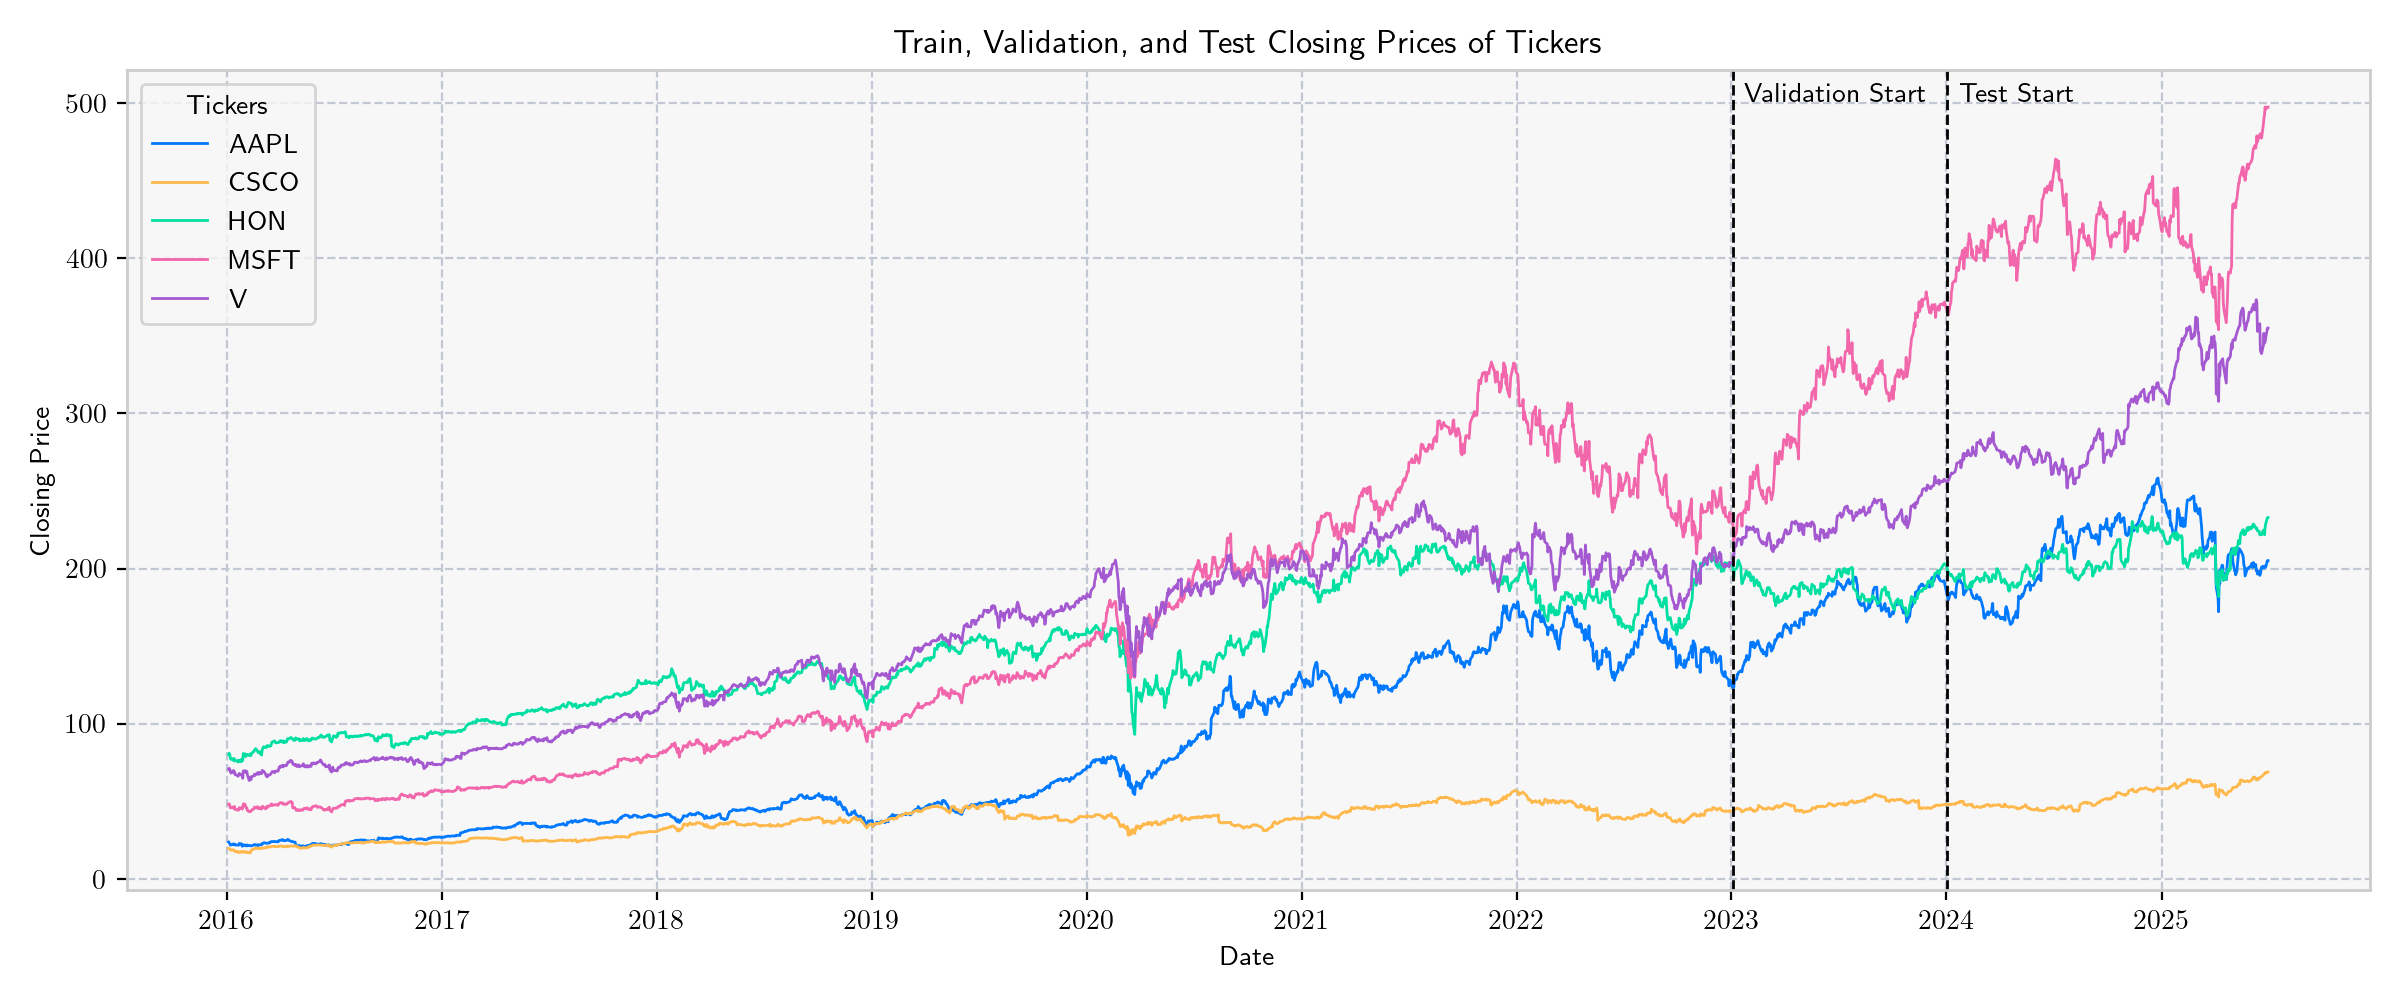
\includegraphics[width=\textwidth]{figures/dataset_split.png}
    \caption{Train-Validation-Test Split for the Hyper-parameter tuning on a sample of five assets from the Dow Jones Industrial Average index.}
    \label{fig:dataset_split}
\end{figure}

The \texttt{wandb} library provides an interactive website to visualise the results of the hyper-parameters in terms of the metric chosen for the optimisation and, if applicable, any other metrics that were chosen to be reported. In this case, the optimisation metric was the Sharpe ratio, as it balances the trade-off between risk and return, and additionally, the cumulative return was also reported. Figure \ref{fig:a2c_hyperparameter_tuning} shows the reported results for the hyper-parameter tuning of the \acrshort{a2c} algorithm. It compares the chosen hyper-parameter with the resulting optimisation metric in the validation set.

\begin{figure}
\centering
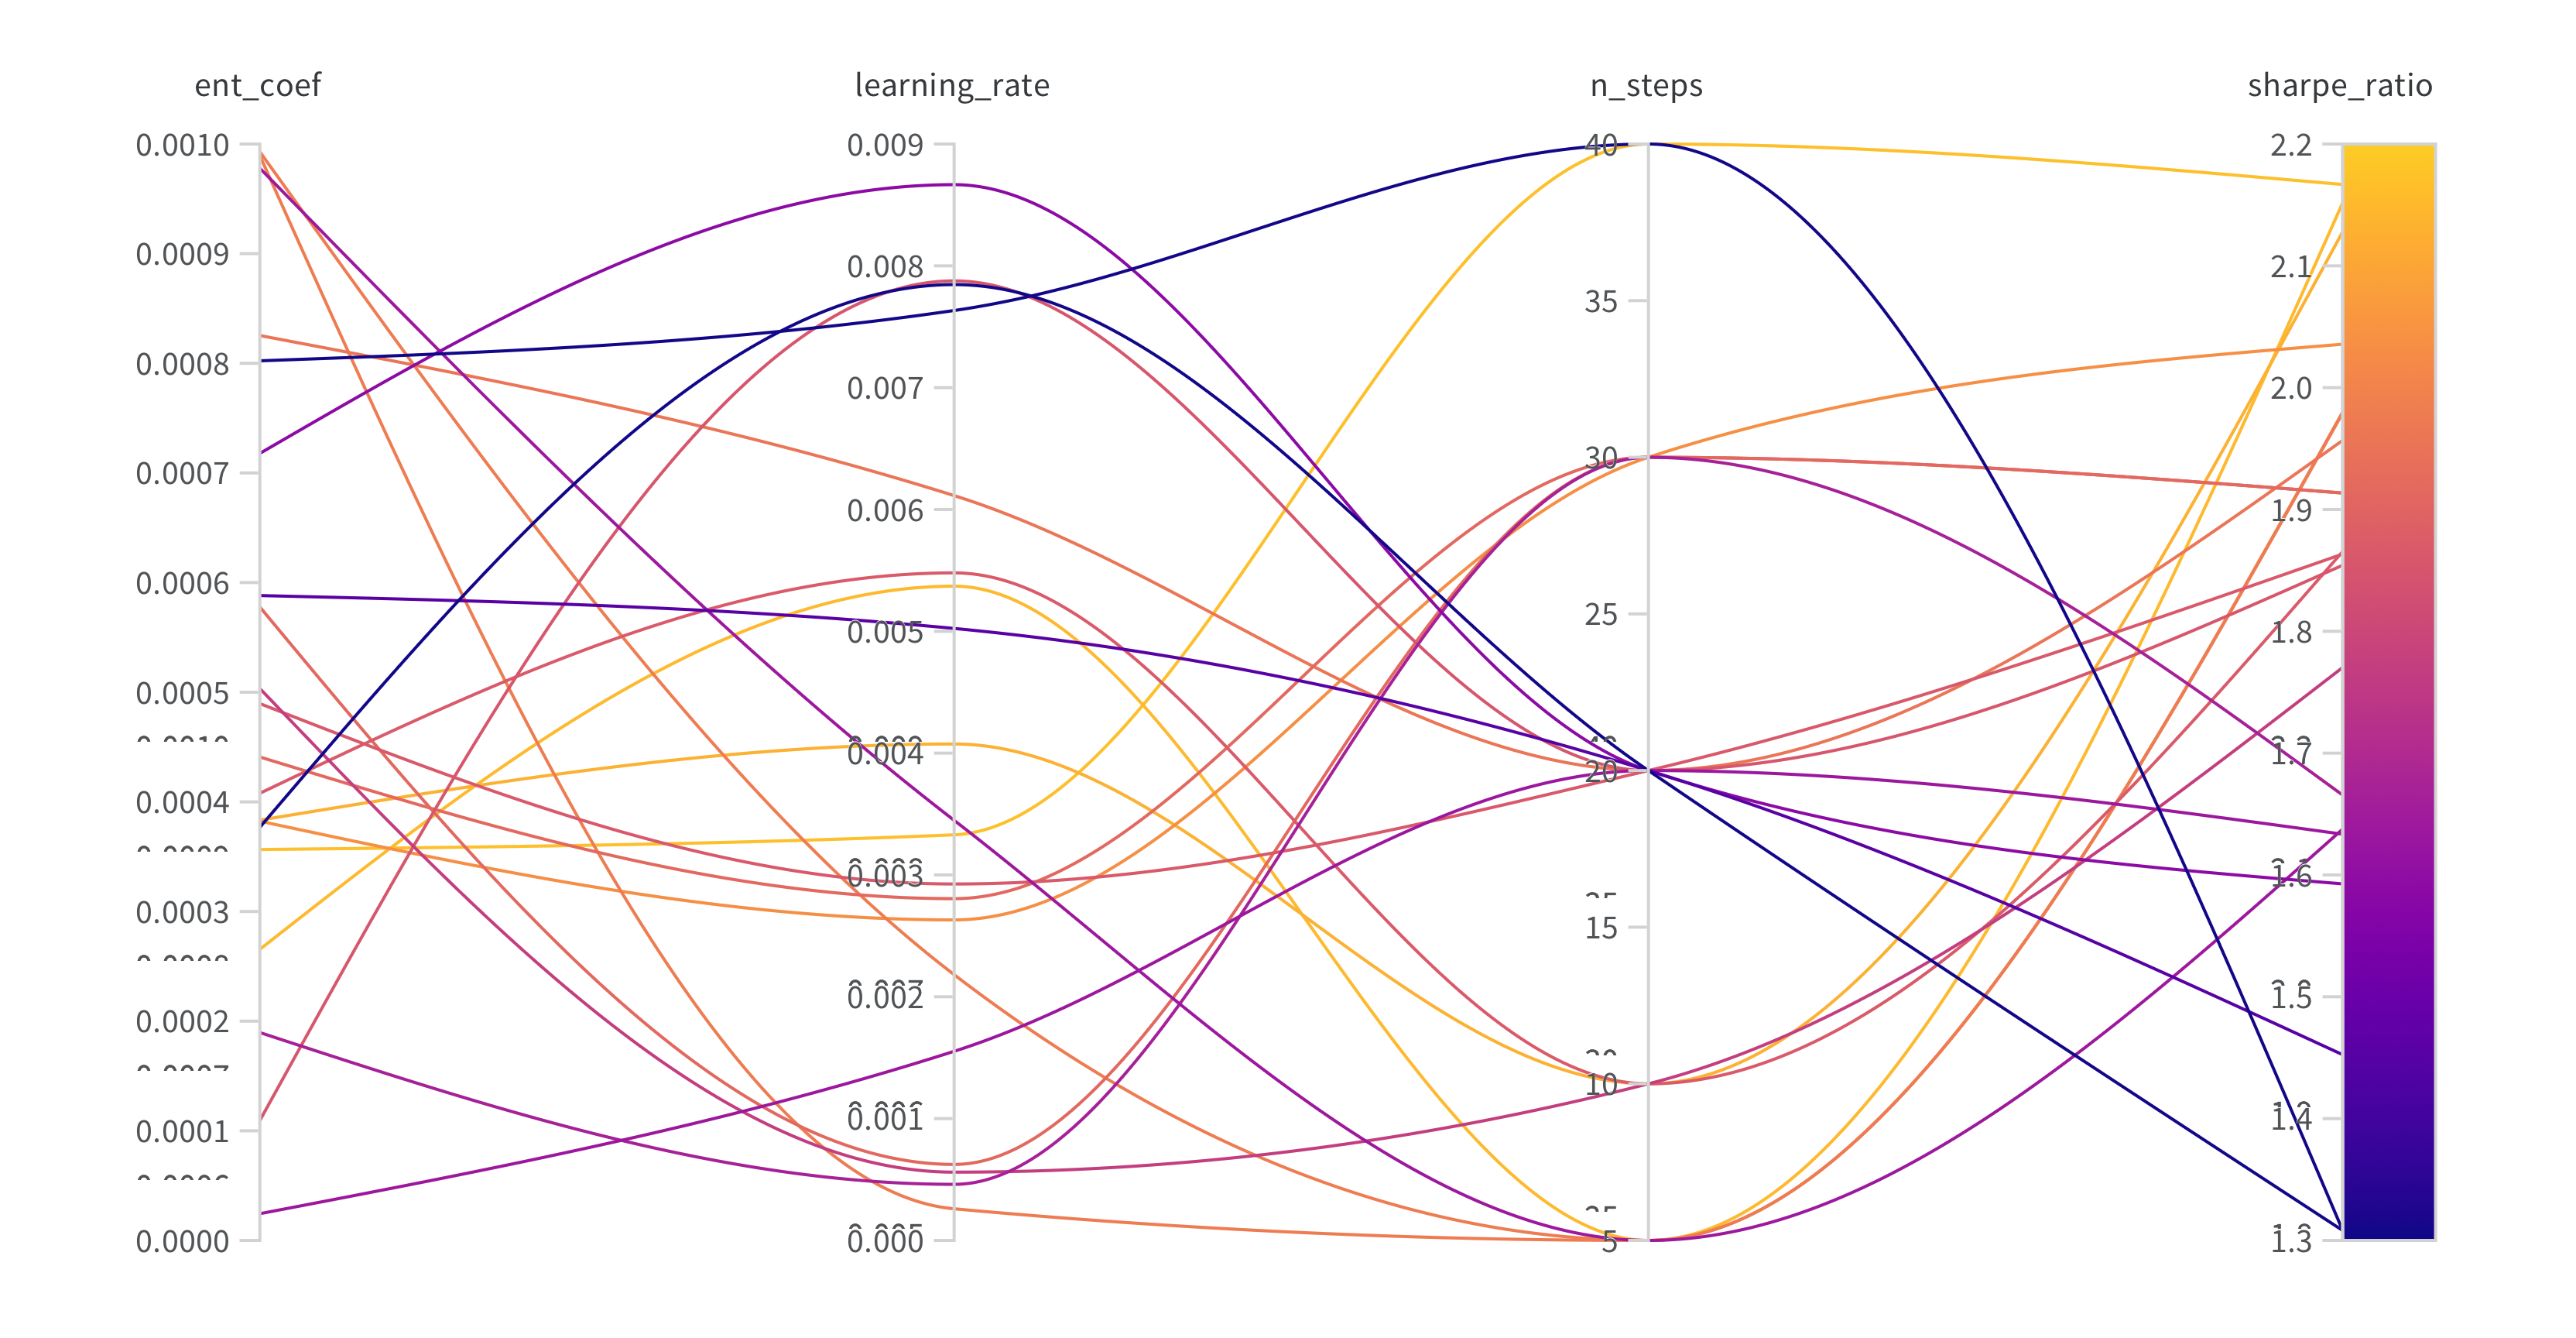
\includegraphics[width=\textwidth]{figures/a2c_hyperparameter_tuning.png}
\caption{Hyper-parameter tuning results for the \acrshort{a2c} algorithm.}
\label{fig:a2c_hyperparameter_tuning}
\end{figure}

The hyper-parameter tuning process was repeated for the other four algorithms, resulting in the hyper-parameters shown in Table \ref{tab:default_hyperparameters}. Since the search had been done in the validation dataset, the best-performing models were evaluated and benchmarked against the test dataset to assess their generalisation performance, whose results are presented in Table \ref{tab:test_results}.

\begin{longtable}{|p{2cm}|p{2.1cm}|p{2.1cm}|p{2.1cm}|p{1.5cm}|p{2cm}|}
    \caption{Results of hyper-parameter tuning on the test dataset.}
    \label{tab:test_results}
    \\ 
    \hline
    \textbf{Dataset} & \textbf{Annualised return} & \textbf{Cumulative return} & \textbf{Annualised volatility} & \textbf{Sharpe ratio} & \textbf{Max drawdown}  \\ \midrule
    \endfirsthead

    \hline
    \textbf{Algorithm / Benchmark} & \textbf{Annualised return} & \textbf{Cumulative return} & \textbf{Annualised volatility} & \textbf{Sharpe ratio} & \textbf{Max drawdown}  \\ \midrule
    \endhead

    \endfoot
    \hline

    \textbf{A2C} & 0.1679 & 0.2598 & 0.1968 & 0.8859 & -0.2186 \\ \hline
    \textbf{PPO} & 0.2158 & 0.3375 & 0.1697 & 1.2364 & -0.1630 \\ \hline
    \textbf{DDPG} & 0.2231 & 0.3494 & 0.1763 & 1.2300 & -0.1684 \\ \hline
    \textbf{TD3} & 0.2174 & 0.3401 & 0.1731 & 1.2227 & -0.1598 \\ \hline
    \textbf{SAC} & 0.1717 & 0.2659 & 0.1762 & 0.9866 & -0.1825 \\ \hline
    \textbf{Mean} & 0.0989 & 0.1503 & 0.1896 & 0.5923 & -0.1972 \\ \hline
    \textbf{Min} & 0.2308 & 0.3609 & 0.1681 & 1.3193 & -0.1559 \\ \hline
    \textbf{Momentum} & 0.1074 & 0.1635 & 0.1868 & 0.6396 & -0.2025 \\ \hline
    \textbf{Equal} & 0.2010 & 0.3123 & 0.1758 & 1.1290 & -0.1762 \\ \hline
\end{longtable}
